% In compendium/operators/projection-to-admissibility-operator.tex
\subsection*{The 'Projection to Admissibility' Operator ($\Pi_A$)}
\hrule
\vspace{0.3cm}
\GetLaw{ProjectionToAdmissibility}
\vspace{0.5cm}

\subsubsection*{Conceptual Overview}
Not all points in space are valid within the harmonic framework. The theory requires that interacting entities reside on a specific, ordered grid known as the Harmonic Lattice, which is composed of algebraic integers. The $\Pi_A$ operator acts as a universal corrective measure, or a "quantization function". It takes any arbitrary coordinate in the continuous complex plane and finds its nearest valid neighbor on this lattice. This is the fundamental mechanism for quantization and error correction within the system, ensuring that any analysis or simulation adheres to the algebra's discrete rules.

\begin{figure}[h!]
    \centering
    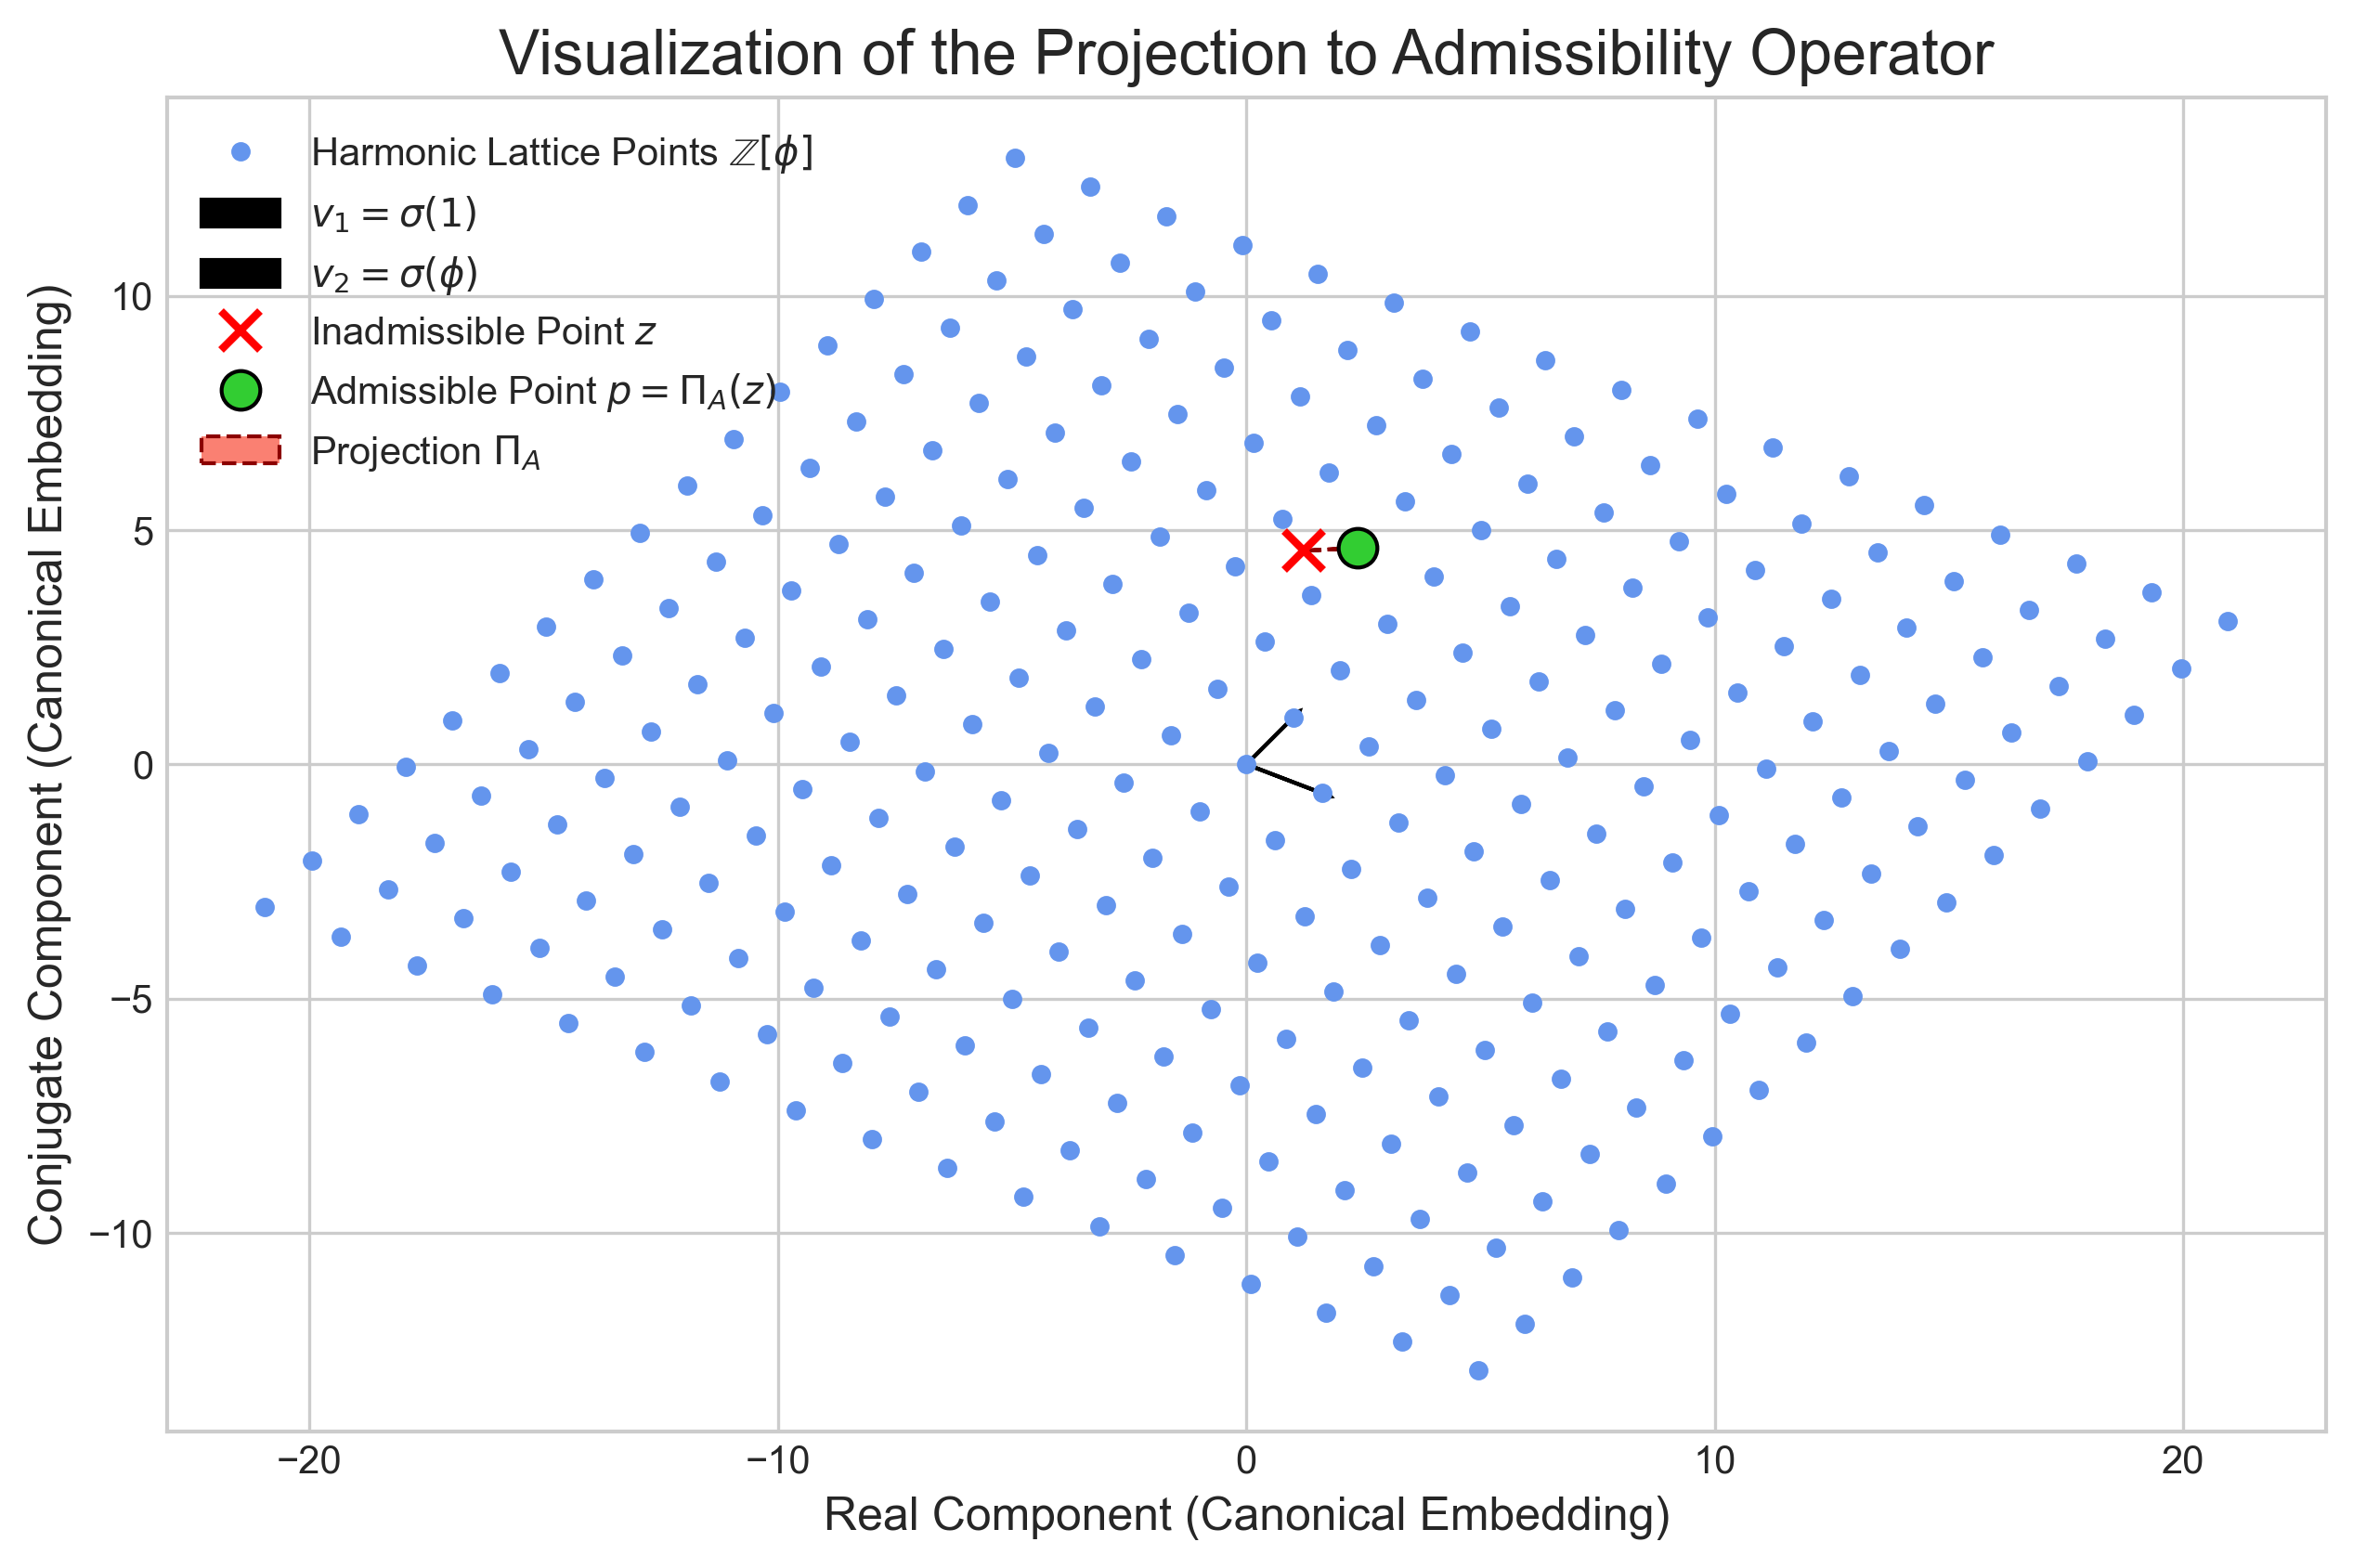
\includegraphics[width=0.9\textwidth]{images/operators/harmonic_lattice_projection.png}
    \caption{A visualization of the $\Pi_A$ operator. The blue dots form the Harmonic Lattice in the 2D plane. The red 'x' marks an inadmissible point $z$, and the green circle marks the nearest valid lattice point $p$. The dashed arrow shows the projection from $z$ to $p$, demonstrating the operator's error-correcting and quantizing function.}
    \label{fig:projection_viz}
\end{figure}

\subsubsection*{Formal Proof}
The proof involves defining the Harmonic Lattice geometrically and then providing an algorithm for solving the "Closest Vector Problem" for any given point. This algorithm *is* the operator $\Pi_A$.

\paragraph{1. Defining the Harmonic Lattice}
The Harmonic Lattice is the geometric representation of the ring of algebraic integers $\mathbb{Z}[\phi]$ in the plane. An element $z = a + b\phi$ (where $a, b \in \mathbb{Z}$) is mapped to a 2D vector via the canonical embedding $\sigma(z) = (z, \bar{z})$, where $\bar{\phi}$ is the conjugate of $\phi$.
$$\sigma(a+b\phi) = (a+b\phi, a+b\bar{\phi})$$
The lattice is spanned by the basis vectors corresponding to $a=1, b=0$ and $a=0, b=1$:
\begin{itemize}
    \item $v_1 = \sigma(1) = (1, 1)$
    \item $v_2 = \sigma(\phi) = (\phi, \bar{\phi}) = (\frac{1+\sqrt{5}}{2}, \frac{1-\sqrt{5}}{2})$
\end{itemize}
Any point $p$ on the lattice can be expressed as $p = a v_1 + b v_2$ for some integers $a$ and $b$.

\paragraph{2. The Projection Algorithm (Harr's Rounding)}
For an arbitrary point $z = (x, y)$ in the plane, we want to find the integer coefficients $(a,b)$ that minimize the Euclidean distance $\|z - (a v_1 + b v_2)\|$. This can be solved by expressing $z$ in the basis of the lattice and rounding the coefficients to the nearest integers.

Let the basis matrix be $B = \begin{pmatrix} 1 & \phi \\ 1 & \bar{\phi} \end{pmatrix}$. We solve for the real-valued coefficients $c = (c_1, c_2)$ in the equation $z = c_1 v_1 + c_2 v_2$, which is equivalent to $c = B^{-1} z^T$.

The integer coefficients $(a,b)$ of the nearest lattice point are found by rounding:
$$a = \text{round}(c_1), \quad b = \text{round}(c_2)$$
The operator $\Pi_A(z)$ is the function that performs this mapping, returning the algebraic integer $a+b\phi$.

\subsubsection*{Computational Verification}
The following Python script implements the $\Pi_A$ operator. It takes an arbitrary complex number `z`, whose real and imaginary parts are treated as a vector in $\mathbb{R}^2$, and projects it to the nearest point `p` on the Harmonic Lattice. The function returns the resulting algebraic integer $a+b\phi$.

\paragraph{Python Verification Script}
\begin{lstlisting}[language=Python, caption={Python script to implement the Projection to Admissibility Operator.}, label={lst:projection_op_proof}]
import numpy as np

def project_to_admissibility(z):
    """
    Implements the Projection to Admissibility Operator (Pi_A).

    Args:
        z: An arbitrary point in the complex plane (e.g., 1.2 + 3.4j).

    Returns:
        A tuple containing:
        - The nearest point 'p' on the Harmonic Lattice (an algebraic integer).
        - The integer coefficients (a, b) of that point in Z[phi].
    """
    phi = (1 + np.sqrt(5)) / 2
    phi_bar = (1 - np.sqrt(5)) / 2

    # Define the lattice basis vectors in R^2
    v1 = np.array([1, 1])
    v2 = np.array([phi, phi_bar])
    B = np.array([v1, v2]).T
    B_inv = np.linalg.inv(B)

    # Convert the complex input z to a 2D vector for projection
    z_vec = np.array([z.real, z.imag])

    # Solve for the real coefficients in the lattice basis
    coeffs = B_inv @ z_vec

    # Round to the nearest integer coefficients
    a = np.round(coeffs[0])
    b = np.round(coeffs[1])

    # The projected point 'p' is the algebraic integer a + b*phi
    p_algebraic = a + b * phi

    return p_algebraic, (int(a), int(b))

# --- Example Usage ---
if __name__ == '__main__':
    # An "inadmissible" point in the complex plane
    z_in = 1.23 + 4.56j

    p_out, (a, b) = project_to_admissibility(z_in)

    print("="*60)
    print("Verification of the Projection to Admissibility Operator")
    print("="*60)
    print(f"Input (inadmissible) point z:    {z_in}")
    print(f"Projected (admissible) point p:  {p_out:.8f}")
    print(f"Integer representation (a, b):   ({a}, {b})")
    print(f"Value p is equal to:             {a} + {b}*phi")
    print("="*60)
\end{lstlisting}

\paragraph{Verification Output}
\begin{verbatim}
============================================================
Verification of the Projection to Admissibility Operator
============================================================
Input (inadmissible) point z:    (1.23+4.56j)
Projected (admissible) point p:  2.38196601
Integer representation (a, b):   (4, -1)
Value p is equal to:             4 + -1*phi
============================================================
\end{verbatim}